\section{The \bench{} Benchmark}
\label{sec:benchmark}

\subsection{Task selection and sources}
\bench{} comprises \textbf{18 tasks}: the A, B, and C problems of CUMCM and of MCM for each of 2023, 2024, and 2025. The two contests are complementary in style---CUMCM problems are engineering/optimization-heavy and stated in Chinese; MCM problems are modeling-flavored and stated in English---and taking all three problems of each year covers the standard ``A = physical/engineering, B = data/optimization, C = data-science'' split without cherry-picking.

Everything is derived from the official contest material. Problem statements are taken from the local corpus (CUMCM: \texttt{cumcm/problems/\{year\}/\{X\}.md}; MCM: \texttt{mcm/problems/\{year\}/\{X\}.md}), and the official attachments (PDFs, \texttt{.xlsx}, \texttt{.csv}) are mirrored verbatim. Table~\ref{tab:tasks} lists the 18 tasks and the outstanding paper each one is anchored to.

\begin{table}[t]
\centering
\small
\caption{The 18 \bench{} tasks and their O-award anchors. ``Final Q'' is the contest question whose numeric core is scored; oracle coverage is 18/18.}
\label{tab:tasks}
\begin{tabular}{@{}lllll@{}}
\toprule
Slug & Contest & Topic & Final Q & O-award \\
\midrule
\texttt{cumcm-2023-a-heliostat-field}   & CUMCM 2023 A & Heliostat field design        & Q3 & A175 \\
\texttt{cumcm-2023-b-multibeam-lines}   & CUMCM 2023 B & Multibeam survey lines        & Q4 & B226 \\
\texttt{cumcm-2023-c-vegetable-pricing} & CUMCM 2023 C & Vegetable pricing/replenish   & Q4 & C050 \\
\texttt{cumcm-2024-a-dragon-dance}      & CUMCM 2024 A & Bench-dragon kinematics       & Q5 & A016 \\
\texttt{cumcm-2024-b-production-decision}& CUMCM 2024 B & Production decisions          & Q4 & B159 \\
\texttt{cumcm-2024-c-crop-planting}     & CUMCM 2024 C & Crop-planting strategy        & Q1 & C038 \\
\texttt{cumcm-2025-a-smoke-screen}      & CUMCM 2025 A & UAV smoke-screen strategy     & Q5 & A196 \\
\texttt{cumcm-2025-b-sic-thickness}     & CUMCM 2025 B & SiC epi-layer thickness       & Q3 & B157 \\
\texttt{cumcm-2025-c-nipt}              & CUMCM 2025 C & NIPT timing / abnormality     & Q4 & C023 \\
\texttt{mcm-2023-a-plant-community}     & MCM 2023 A & Drought plant communities     & final & 2309229 \\
\texttt{mcm-2023-b-maasai-mara}         & MCM 2023 B & Maasai Mara land use          & final & 2315379 \\
\texttt{mcm-2023-c-wordle}              & MCM 2023 C & Predicting Wordle results     & final & 2307946 \\
\texttt{mcm-2024-a-lamprey}             & MCM 2024 A & Sex ratios / resource supply  & final & 2407093 \\
\texttt{mcm-2024-b-submersible-search}  & MCM 2024 B & Submersible search            & Q4 & 2419984 \\
\texttt{mcm-2024-c-tennis-momentum}     & MCM 2024 C & Momentum in tennis            & Q5 & 2401298 \\
\texttt{mcm-2025-a-stair-wear}          & MCM 2025 A & Stair wear / footfall         & Q8 & 2501909 \\
\texttt{mcm-2025-b-juneau-tourism}      & MCM 2025 B & Sustainable tourism (Juneau)  & Q3 & 2504448 \\
\texttt{mcm-2025-c-olympic-medals}      & MCM 2025 C & Olympic medal models          & final & 2505964 \\
\bottomrule
\end{tabular}
\end{table}

\subsection{Construction pipeline}
Each task is generated by a build script that is reproducible from the source corpus. The generated directory has a fixed shape:
\begin{itemize}[leftmargin=1.4em,itemsep=1pt]
\item \texttt{instruction.md} --- the prompt. It contains the verbatim contest statement, each cited figure embedded inline, a note giving the in-container figure paths, and a ``Required Benchmark Artifact'' section naming the output file. It ends with the time limit.
\item \texttt{environment/} --- the agent container: a Dockerfile (\texttt{python:3.12-slim} plus a fixed scientific-Python environment) and \texttt{data/}, holding \texttt{problem.md}, \texttt{output\_schema.json}, \texttt{source\_manifest.json}, an \texttt{attachments/} flat mirror with an \texttt{INDEX.md}, a \texttt{repo/} full-path mirror of the original corpus, and any \texttt{figures/}.
\item \texttt{tests/} --- the verifier (a separate container): \texttt{test.sh}, \texttt{test\_outputs.py}, \texttt{score\_result.py}, plus the scoring panel \texttt{score\_config.json}, the anchor \texttt{expected\_result.json}, and auxiliary checks.
\item \texttt{solution/} --- the oracle: \texttt{solve.sh} and \texttt{oracle/}, which contains a runnable reproduction of the anchored O-award paper.
\end{itemize}

\paragraph{Figures are load-bearing.} For problems whose statements cite figures, the figures are cropped from the official PDF---artwork plus its own caption, without surrounding prose---and delivered both inline in the statement and at stable container paths. \textbf{21 unique figures} across 6 tasks (CUMCM 18, MCM 3) are delivered this way; the remaining 12 tasks have no figure. This matters because a text-only agent cannot see them (Figure~\ref{fig:official-fig}), which is exactly what the multimodal comparison in Section~\ref{sec:results} exploits.

\begin{figure}[t]
\centering
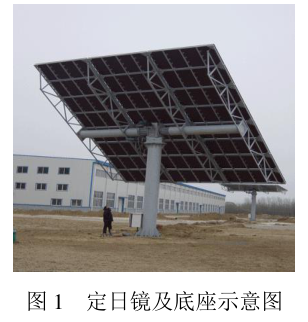
\includegraphics[width=0.62\linewidth]{figures/heliostat_statement_fig1.png}
\caption{An official statement figure, cropped from the CUMCM 2023 A PDF (artwork plus its own caption, without surrounding prose) and delivered inline in the prompt. 21 such figures across 6 tasks are load-bearing: a text-only agent cannot read them.}
\label{fig:official-fig}
\end{figure}

\paragraph{No train/test split.} \bench{} is a pure evaluation set. There is no training partition, no held-out split, and no difficulty tiering: the 18 tasks are evaluated uniformly. This is deliberate for a benchmark of this kind and is stated explicitly in Appendix~\ref{app:dataset}.

\subsection{The artifact contract}
The single scored object is one JSON file per task. Its expected shape is shipped to the agent as \texttt{output\_schema.json} (field names and types only, no values), and the agent is told the exact path (\texttt{/root/results/<slug>\_result.json}). Supplementary CSV/XLSX/PNG artifacts may be written but are not scored. Restricting scoring to a schema-constrained JSON is what makes an automated, reproducible score possible at all; the cost is that the agent must map a free-form modeling effort onto a small set of named numeric fields, which we revisit in Section~\ref{sec:analysis}.

\subsection{Oracle anchors}
Each task is anchored to one outstanding (O-award) paper, re-implemented as a runnable script that reads the official attachments and emits the same artifact JSON. The reproduction is used as the normalization endpoint (\oeval{} $=100\%$), and its per-metric values initialize the scoring panel. Oracle coverage is \textbf{18/18}: every task ships \texttt{solution/oracle/} and an \texttt{expected\_result.json}.

We are explicit about two consequences. First, an anchor is a \emph{reproduction} of one team's choices, not an optimum; Section~\ref{sec:scoring} explains how scoring is designed so that beating the anchor is not punished. Second, reproductions can themselves be wrong. We found and corrected one such case---the dragon-dance final answer---and we treat anchor provenance as a first-class field (each reproduction records its paper id, OCR/PDF source, and a \texttt{reproduction\_scope}). Appendix~\ref{app:baselines} lists the anchors; Section~\ref{sec:analysis} quantifies the anchor-related failure modes.
